\documentclass[11pt,a4paper]{article}
\usepackage[T1]{fontenc}\usepackage[utf8]{inputenc}\usepackage{lmodern,amsmath,amssymb,graphicx,booktabs,array,microtype,float,placeins,listings,xcolor,caption}
\usepackage[margin=25mm]{geometry}\usepackage[hidelinks]{hyperref}\usepackage{fancyhdr}
\pagestyle{fancy}\fancyhf{}\fancyhead[L]{Arduino Thermistor Temperature Measurement}\fancyfoot[C]{\thepage}\setlength{\headheight}{14pt}
\setlength{\parindent}{0pt}\setlength{\parskip}{6pt}\captionsetup{font=small,labelfont=bf}
\lstset{basicstyle=\ttfamily\scriptsize,breaklines=true,columns=fullflexible,keepspaces=true,showstringspaces=false,numbers=left,numberstyle=\tiny\color{gray},frame=single,rulecolor=\color{gray!30}}
\begin{document}
\begin{titlepage}\centering

\includegraphics[height=23mm]{figures/rId9.png}\hfill
\includegraphics[height=23mm]{figures/rId8.png}\par
\vspace{20mm}{\Large Measurement Systems and Laboratory\par}\vspace{10mm}
{\huge\bfseries Thermistor Calibration and Arduino Temperature Measurement\par}\vspace{7mm}
{\Large Laboratory Session Six\par}\vspace{17mm}
Group 15\par\vspace{5mm}{\Large Pouya Asghari\par Amir Mehdi Golchin\par}
\vfill School of Mechanical Engineering\par College of Engineering, University of Tehran\par
First semester of academic year 1404--1405 (Iranian calendar)\par
\end{titlepage}
\section*{About this translation}
This edition translates the supplied Persian report into English and provides editable LaTeX. It retains the calibration data, reported fit, equations, figures, and code listings. Student numbers are omitted. The source's second author name is transliterated as Amir Mehdi Golchin; the preferred Latin spelling should be confirmed.

Original numerical and circuit statements are retained with clearly separated editorial notes. In particular, the calibration resistance formula has a sign error and the fourth LM324 output pin is misstated. The source code is archived unchanged; it has not been uploaded to hardware or executed in MATLAB during preparation.
\begingroup\small\setlength{\parskip}{0pt}\tableofcontents\endgroup\clearpage


\section{Temperature Measurement Experiment}

The objective of this assignment is to build and calibrate a temperature measurement system using a thermistor. A thermistor is a resistor whose resistance changes with temperature. NTC and PTC thermistors have negative and positive temperature coefficients, respectively: their resistance decreases or increases as temperature rises. The thermistor used in this experiment is an NTC device, shown below.

\begin{figure}[H]\centering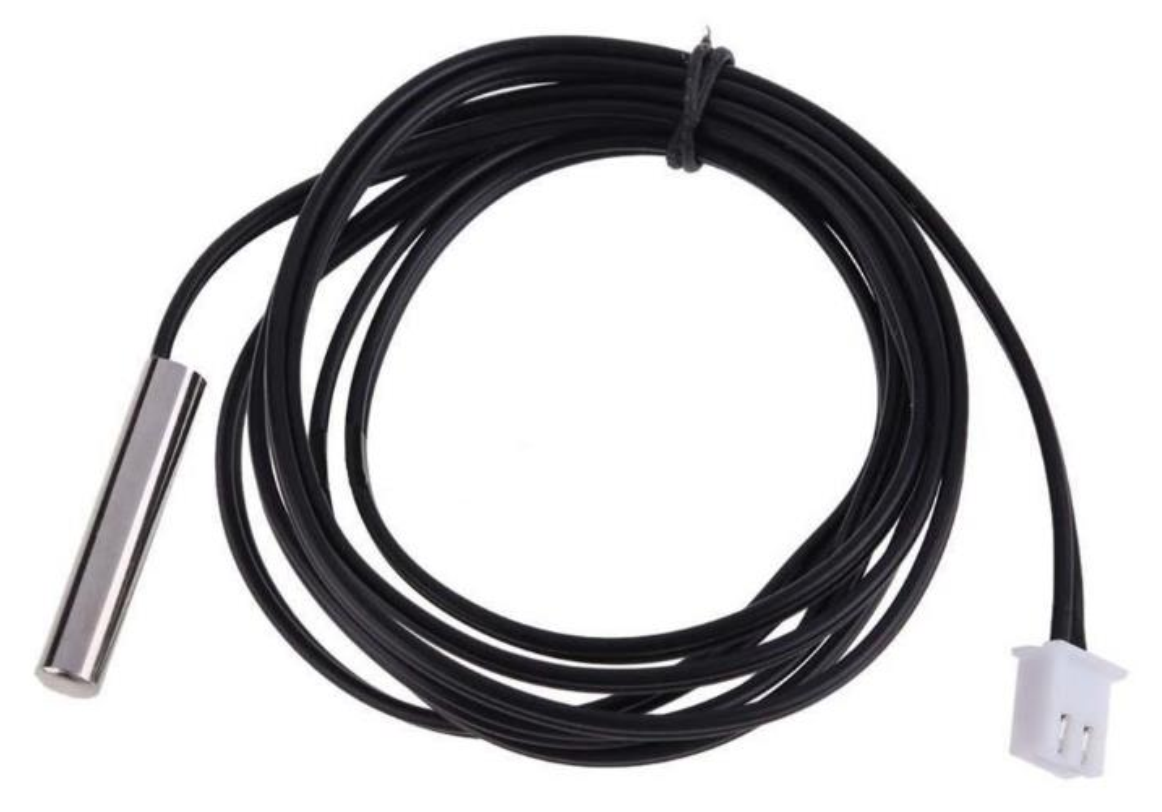
\includegraphics[width=0.92\linewidth,height=0.43\textheight,keepaspectratio]{figures/rId15.png}\caption{Waterproof NTC thermistor.}\end{figure}

\subsection{Calibration}

This section presents the calculations and measurements used to calibrate the thermistor and determine its resistance--temperature relationship. The model is

\[R=R_0\exp\left[B\left(\frac{1}{T}-\frac{1}{T_0}\right)\right].\]

Here, $T_0$ and $R_0$ are the reference temperature and resistance at room temperature ($25^\circ$C), expressed in kelvin and ohms. Calibration is required to determine $B$ and $R_0$. A thermometer and a water-filled beaker are used to record temperature alongside the thermistor resistance obtained from the Arduino calibration circuit and program. Measurements are taken at seven stages while gradually increasing the water temperature. The setup is shown below.

\begin{figure}[H]\centering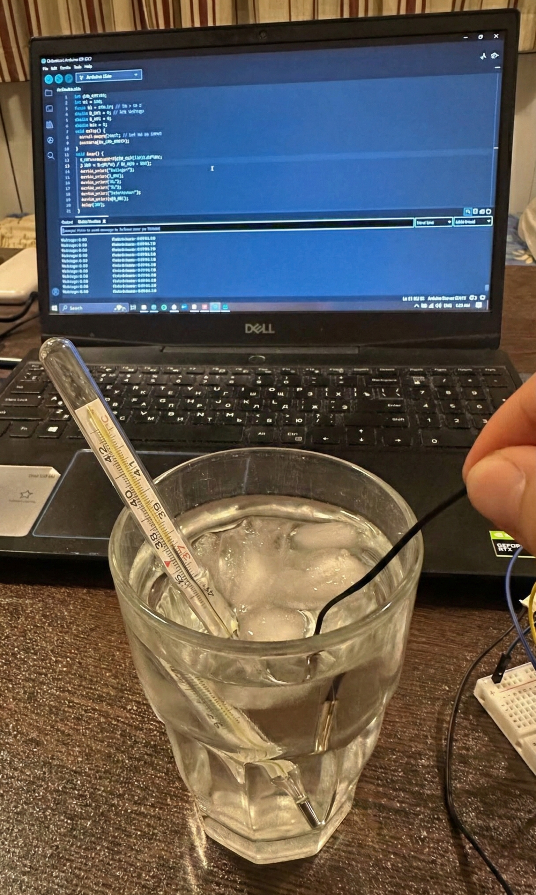
\includegraphics[width=0.92\linewidth,height=0.43\textheight,keepaspectratio]{figures/rId16.png}\caption{Experimental calibration setup.}\end{figure}

The corresponding temperature and resistance measurements are listed in Table 1.

\begin{table}[H]\centering\caption{Measured calibration data.}\begin{tabular}{rr}\toprule Temperature ($^\circ$C) & Resistance ($\Omega$)\\\midrule
3&28034\\12&18419\\25&9637\\33&6998\\42&4915\\55&3117\\70&1890\\\bottomrule\end{tabular}\end{table}

The MATLAB Curve Fitter tool is used to fit the exponential thermistor model to the data in Table 1 and determine $B$ and $R_0$. The source reports the following fitted coefficients and goodness of fit.

\textbf{Fitted constants}

$B=3891.5751$ K.

$R_0=9953.4133\ \Omega$.

Coefficient of determination: $R^2=0.9995$.

\begin{figure}[H]\centering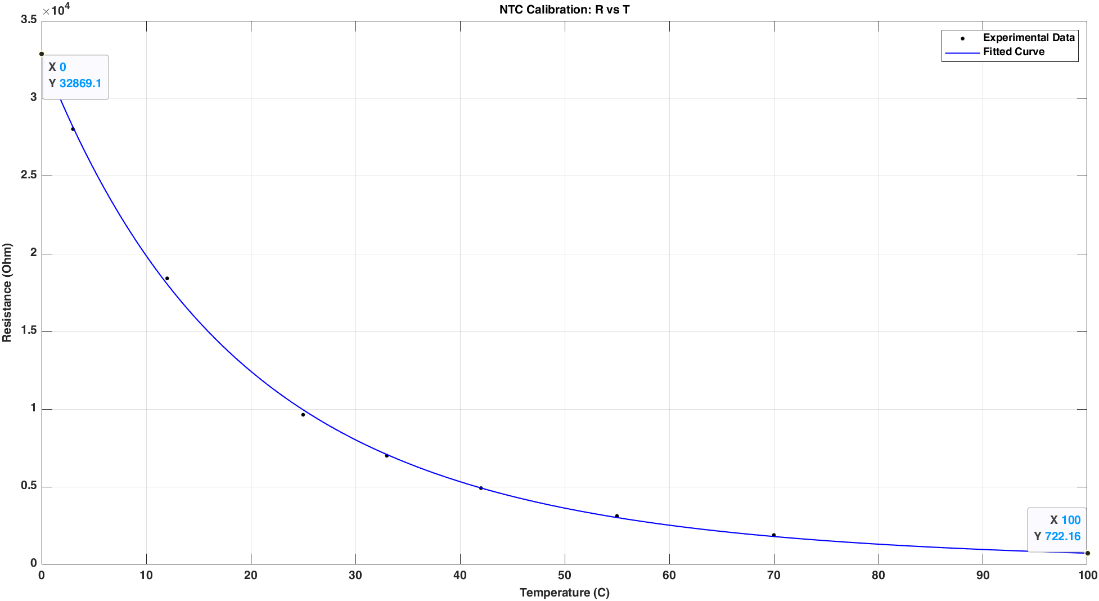
\includegraphics[width=0.92\linewidth,height=0.43\textheight,keepaspectratio]{figures/rId17.png}\caption{Thermistor calibration curve.}\end{figure}

The rounded coefficients adopted are $B=3892$ K and $R_0=9953\ \Omega$. The nominal reference resistance is expected to be $10000\ \Omega$. The fitted value is considered acceptable within the thermistor's stated 5\% tolerance.

The calibration circuit is a voltage divider containing a 10 k$\Omega$ fixed resistor and the thermistor. The midpoint voltage is read at A1. The source gives the following equations for recovering thermistor resistance.

\[V_{\mathrm{out}}=V_{A1}=\frac{R_{\mathrm{NTC}}}{R_{\mathrm{NTC}}+R}V_{\mathrm{in}}=\frac{R_{\mathrm{NTC}}}{R_{\mathrm{NTC}}+10^4}(5\ \mathrm{V}).\]

\[R_{\mathrm{NTC}}=\frac{V_{\mathrm{out}}10^4}{V_{\mathrm{out}}-5},\qquad V_{\mathrm{out}}=\frac{N_{A1}}{1023}(5\ \mathrm{V}).\]

The Arduino calibration program performs these calculations at each temperature and prints the corresponding resistance to the Serial Monitor. The voltage-divider circuit is shown below. The sign of the source's resistance formula is reviewed in the editorial appendix.

\begin{figure}[H]\centering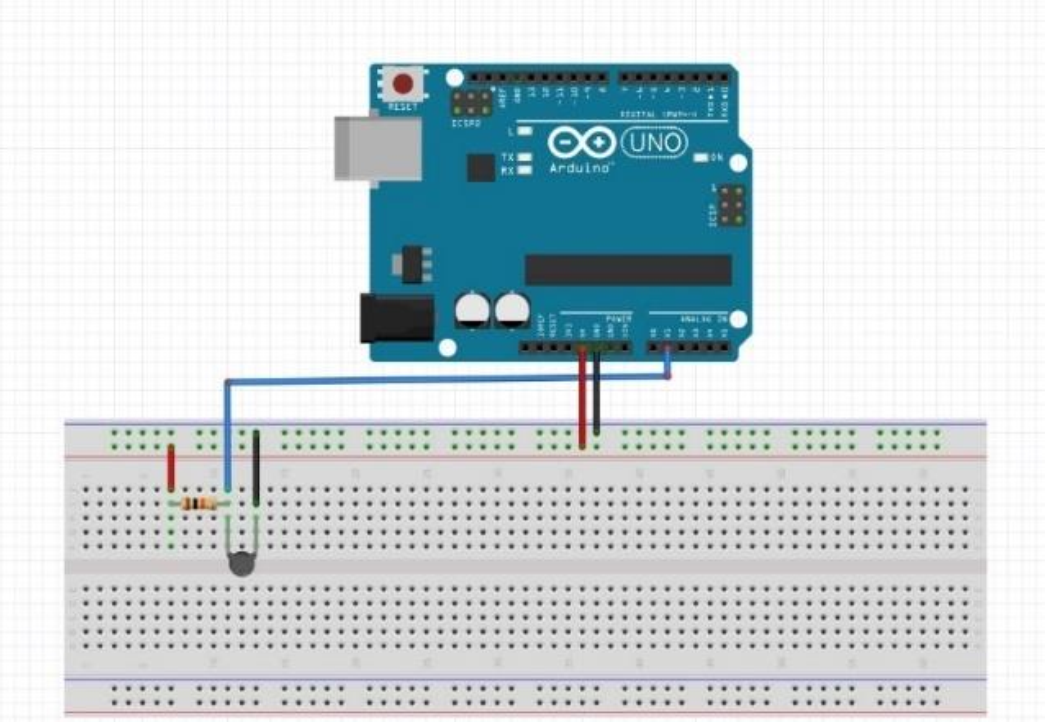
\includegraphics[width=0.92\linewidth,height=0.43\textheight,keepaspectratio]{figures/rId18.png}\caption{Voltage divider used for calibration.}\end{figure}

\subsection{Implementation of the temperature measurement system}

The first design step is to calculate the parameters intended to improve the measurement resolution. The thermistor voltage at $0^\circ$C is obtained from the fitted resistance model and voltage-divider relation. This voltage is used as an offset so that the measurement range starts near zero volts at $0^\circ$C.

\[R(0^\circ\mathrm{C})=32869.1\ \Omega,\qquad V_0=\frac{32869.1}{32869.1+10^4}(5\ \mathrm{V})\approx3.83\ \mathrm{V}.\]

A differential operational-amplifier circuit is used to subtract the two signals. Its voltage--temperature characteristic is shown below.

\begin{figure}[H]\centering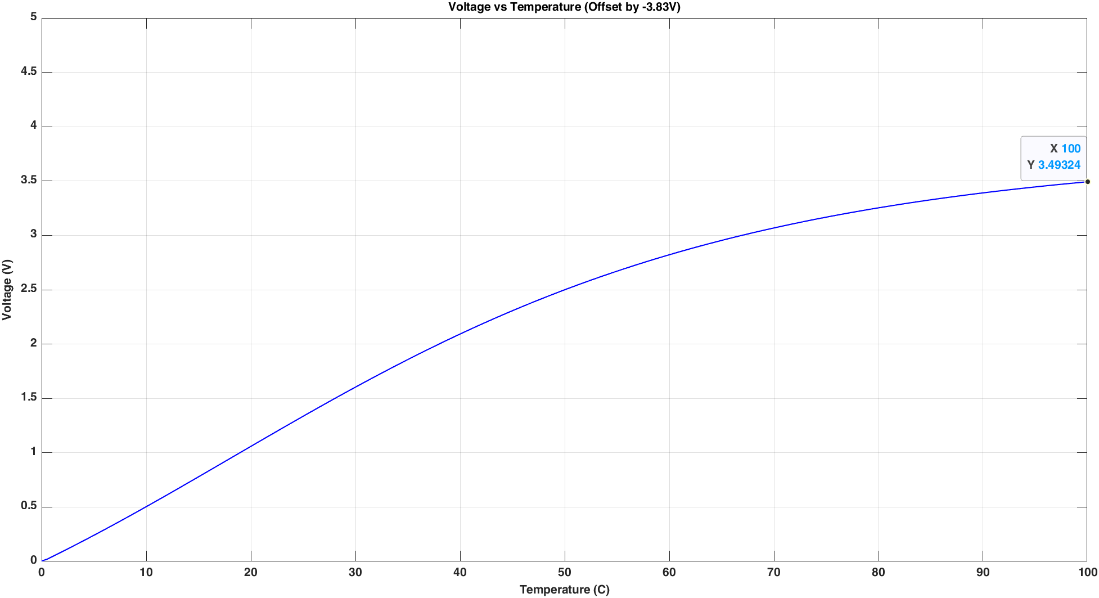
\includegraphics[width=0.92\linewidth,height=0.43\textheight,keepaspectratio]{figures/rId19.png}\caption{Voltage versus temperature after the proposed differential offset.}\end{figure}

The source proposes reducing the ADC upper reference from 5 V to 3.49 V, distributing the available ADC codes across a narrower voltage range to improve resolution. In addition to the differential circuit, the Arduino AREF voltage is adjusted using a potentiometer.

The implementation uses the high-impedance differential-amplifier circuit presented in the LM324 datasheet.

\begin{figure}[H]\centering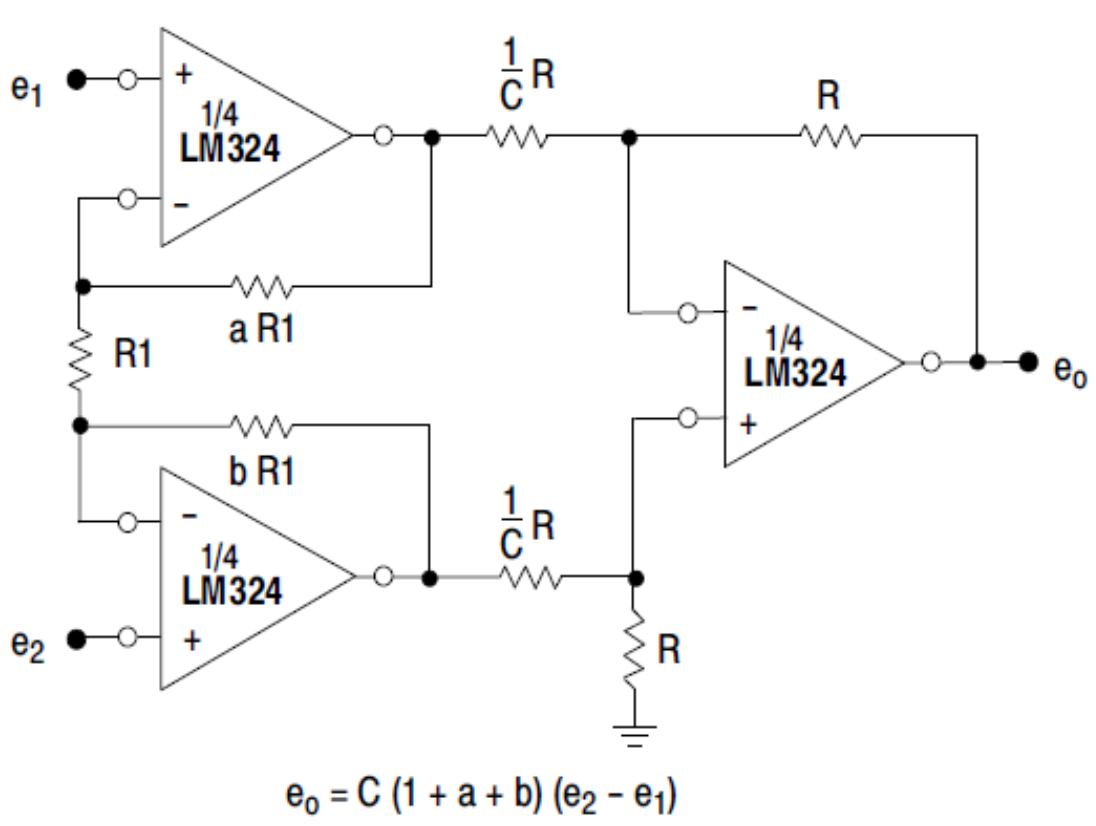
\includegraphics[width=0.92\linewidth,height=0.43\textheight,keepaspectratio]{figures/rId20.png}\caption{High-impedance differential-amplifier topology.}\end{figure}

According to the circuit's expression, setting $a=b=0$ and $1/C=1$ yields only the difference between input signals $e_1$ and $e_2$, without additional gain. This arrangement is used to reduce loading and address impedance matching. The source describes a simple differential circuit with larger resistors, such as 100 k$\Omega$ or 1 M$\Omega$, as an alternative to the 10 k$\Omega$ implementation.

Operational-amplifier sections 1, 2, and 4 of the LM324 are used. The pinout and the circuit based on this configuration are shown below. The original text cross-references Figure 2 here; the relevant amplifier topology is the high-impedance circuit reproduced above.

\begin{figure}[H]\centering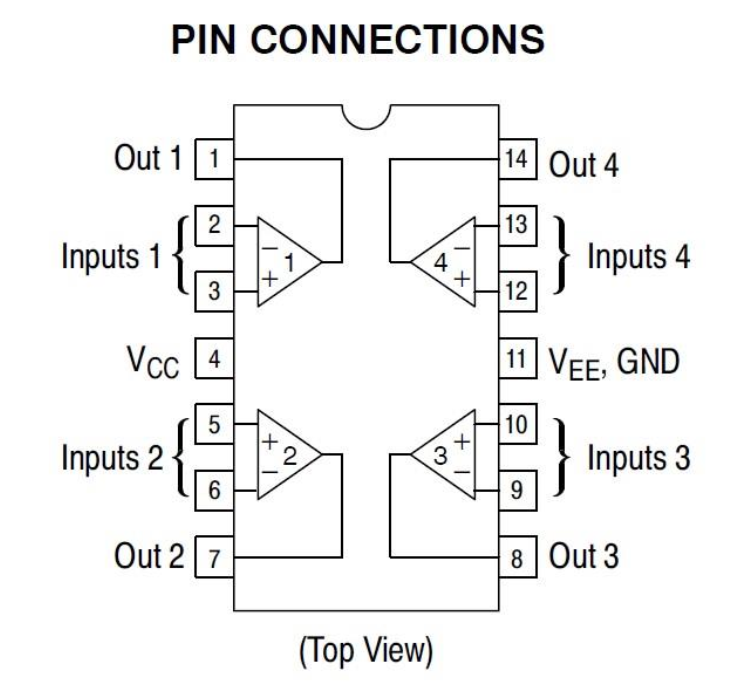
\includegraphics[width=0.92\linewidth,height=0.43\textheight,keepaspectratio]{figures/rId21.png}\caption{LM324 pin connections.}\end{figure}

The circuit is first drawn by hand.

\begin{figure}[H]\centering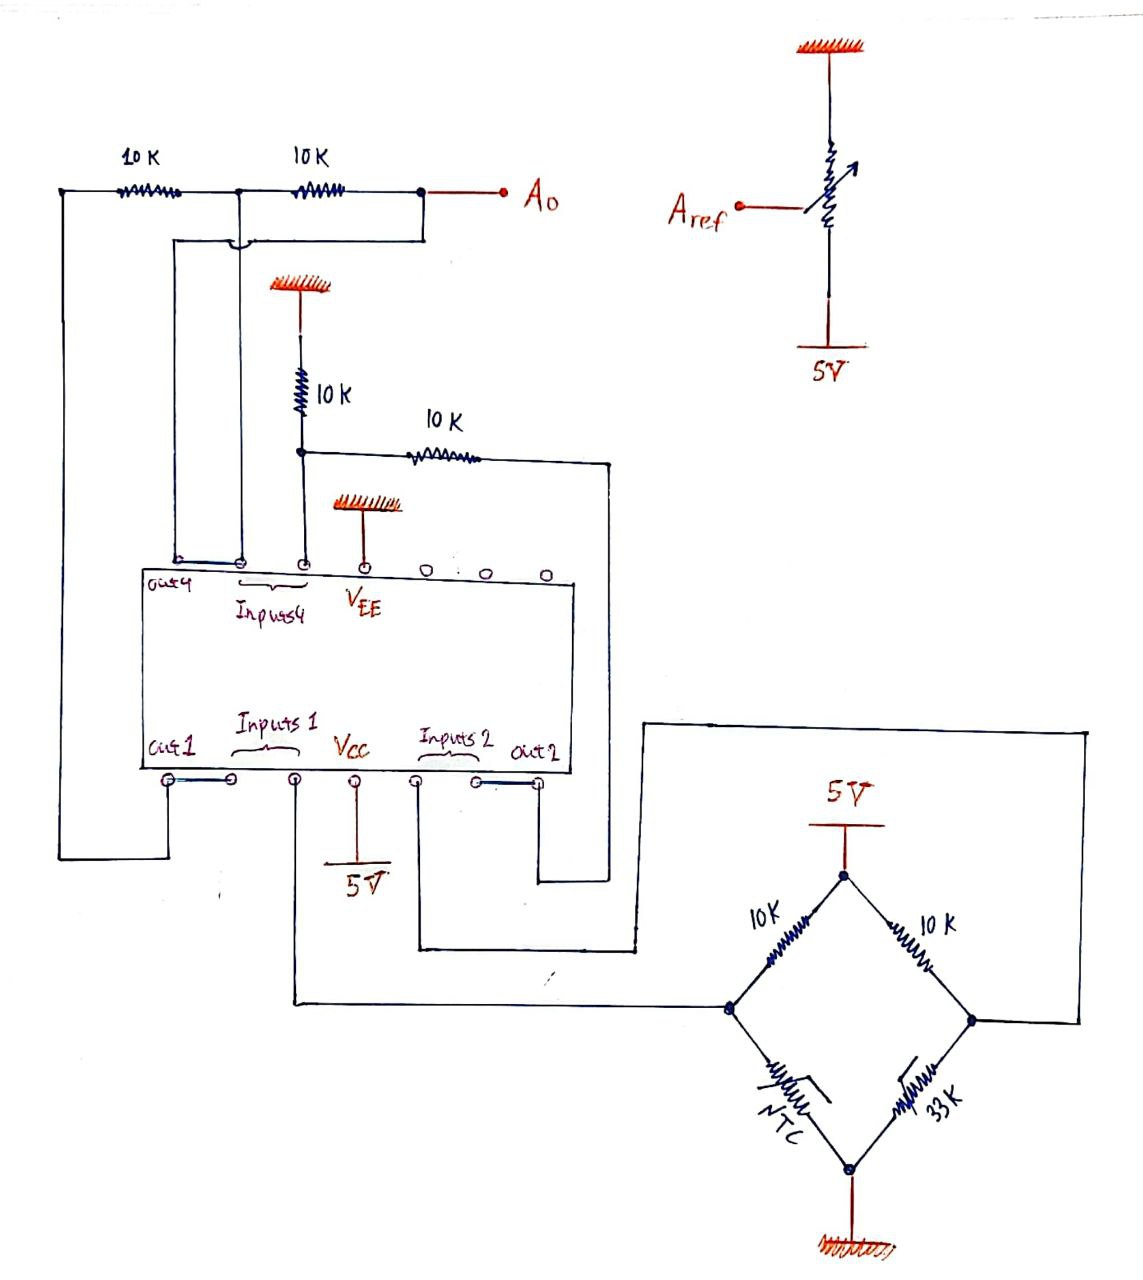
\includegraphics[width=0.92\linewidth,height=0.43\textheight,keepaspectratio]{figures/rId22.png}\caption{Hand-drawn differential-amplifier circuit.}\end{figure}

A Fritzing circuit representation is then prepared. The original source describes this as a simulation; no native Fritzing project or simulated electrical dataset is included in the archive.

\begin{figure}[H]\centering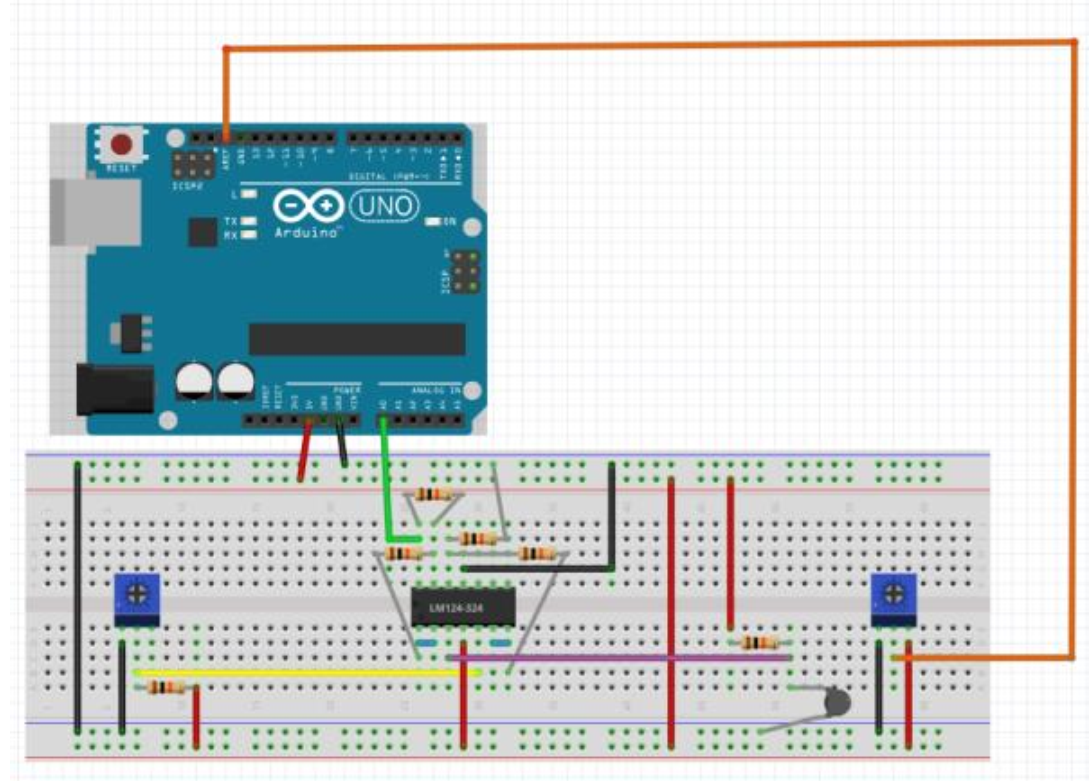
\includegraphics[width=0.92\linewidth,height=0.43\textheight,keepaspectratio]{figures/rId23.png}\caption{Fritzing representation of the circuit.}\end{figure}

As the thermistor temperature changes, its resistance changes, and the voltage divider converts that resistance to a voltage. This voltage enters the first buffer at pin 3. A second divider, comprising a 10 k$\Omega$ resistor and a 50 k$\Omega$ potentiometer adjusted to approximately $32869\ \Omega$, generates the fitted $0^\circ$C reference of 3.83 V and feeds the second buffer at pin 5. These signals are applied to the inverting and noninverting inputs of the fourth LM324 section at pins 13 and 12. The source states that the difference is read from pin 1 using Arduino A0; the correct fourth-section output pin is discussed in the editorial appendix. All fixed resistors in the implemented amplifier circuit are 10 k$\Omega$. A 10 k$\Omega$ potentiometer sets the Arduino AREF voltage. Its nominal divider setting is calculated below.

\[\frac{R}{10^4}(5\ \mathrm{V})=3.49\ \mathrm{V}\quad\Longrightarrow\quad R=6980\ \Omega.\]

\begin{figure}[H]\centering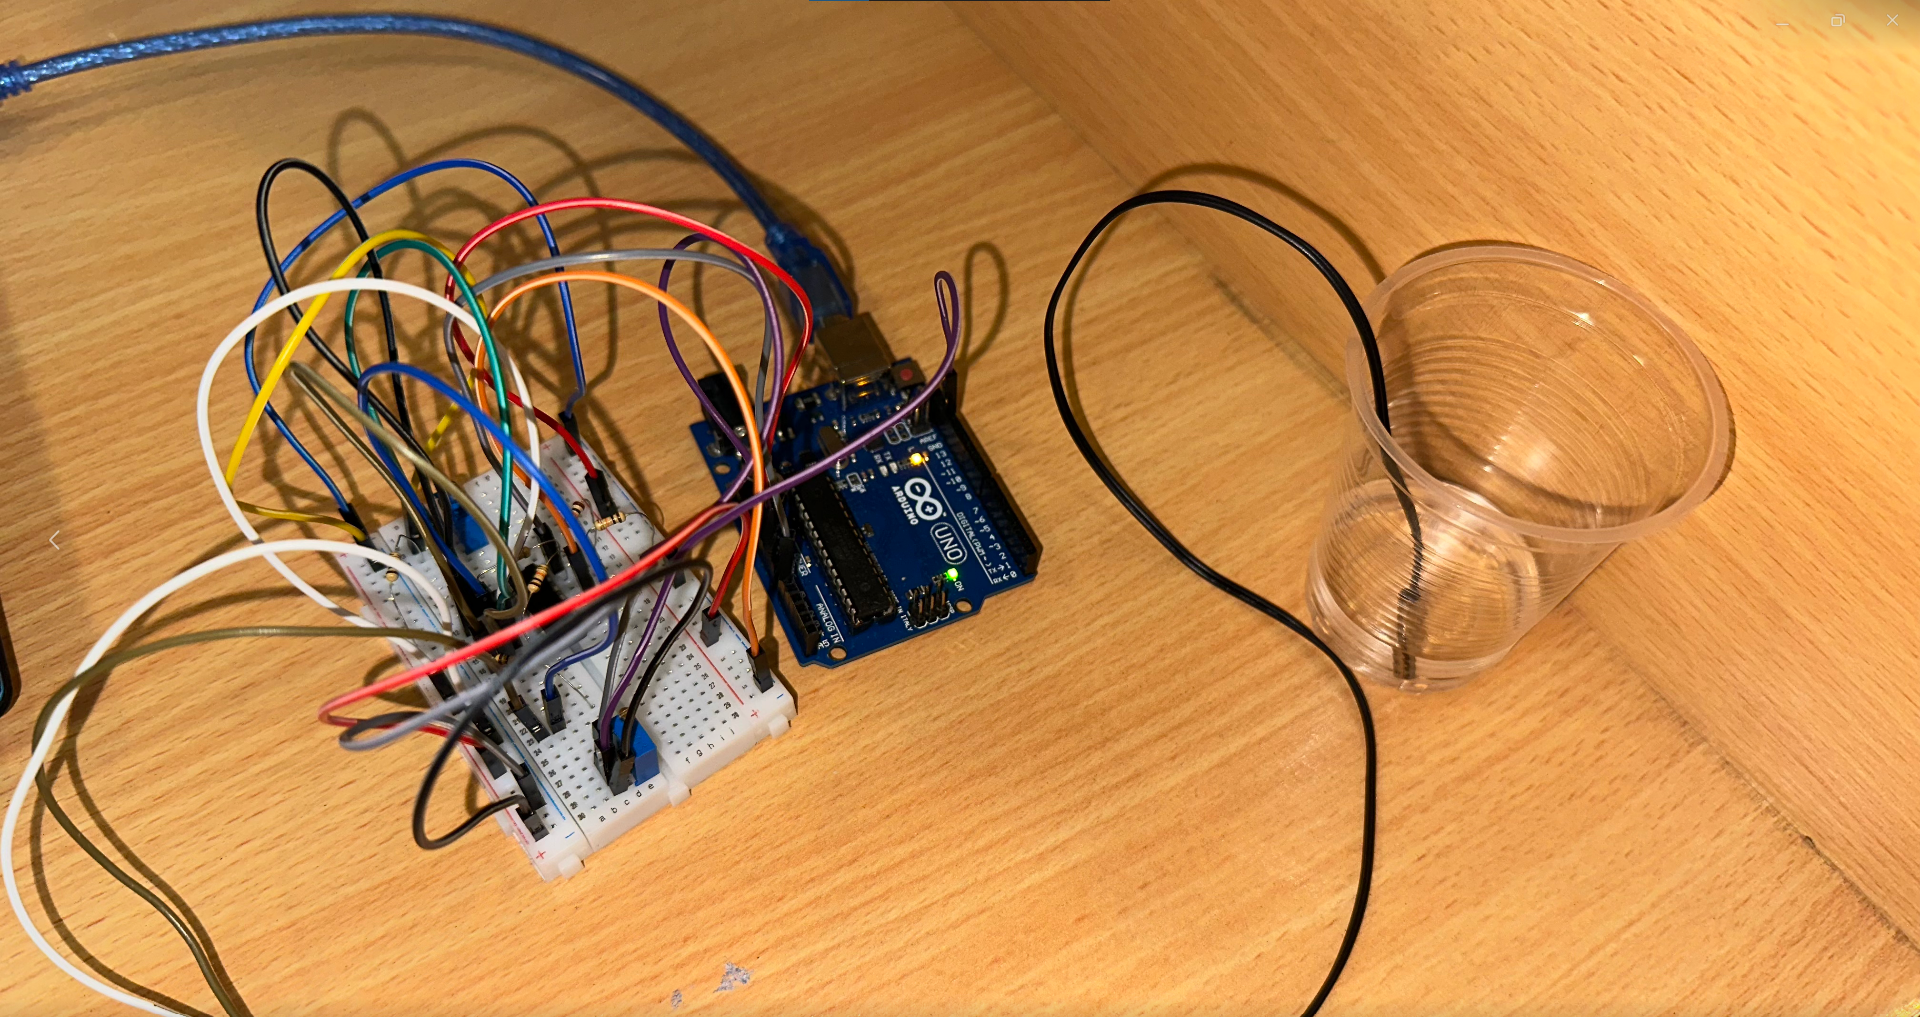
\includegraphics[width=0.92\linewidth,height=0.43\textheight,keepaspectratio]{figures/rId24.png}\caption{Assembled temperature measurement circuit.}\end{figure}

\subsection{Code explanation}

The MATLAB code fits the thermistor resistance model to the calibration data using Curve Fitter functionality. The source describes the fitted relationship as a function named CalCurve. It then calculates reference resistances for the circuit, called a Watson bridge in the source, and the ADC reference adjustment, using variables described as R0 and Rref. Calibration and original/offset voltage--temperature curves are plotted. The supplied Live Script implements the fit directly; it does not contain a separate CalCurve function or an Rref calculation.

In the calibration sketch, the voltage divider is read at A1 and mapped to a voltage between 0 and 5 V, stored as V\_NTC. The thermistor resistance is calculated and stored as R\_NTC, then voltage and resistance are printed to the Serial Monitor. Although the original text calls A1 a digital pin, it is used here as an analog ADC input.

In the temperature measurement sketch, the differential-amplifier output is read at A0 at a nominal sampling frequency of 5 Hz using the Sampling interrupt callback. The voltage is stored as V\_NTC. The resistance is recovered from the differential output and the 3.83 V offset, then converted to temperature using the fitted thermistor relationship. Voltage, resistance, and temperature are printed to the Serial Monitor.

\FloatBarrier\appendix\section{Original Code Listings}
The native Arduino files are included unchanged. The MATLAB text file is extracted from the supplied Live Script and reproduces its executable text.
\subsection{Arduino calibration sketch}
\lstinputlisting[language=C++]{../arduino/Calibration/Calibration.ino}
\subsection{MATLAB calibration and plotting}
\lstinputlisting[language=Matlab]{../matlab/calibrate_ntc.m}
\subsection{Arduino temperature measurement sketch}
\lstinputlisting[language=C++]{../arduino/sketch_feb15a/sketch_feb15a.ino}
\section{Original References}
\begin{enumerate}
\item Measurement Systems Laboratory, Session Six instructions, School of Mechanical Engineering, University of Tehran. The instructions were not supplied as a separate file.
\item \url{https://www.electronics-tutorials.ws/filter/filter2.html}. URL retained from the source reference list; the source does not provide a full citation.
\end{enumerate}
\section{Editorial Review and Reproduction Notes}
\subsection{Calibration equation sign}
For the stated divider relation $V=V_{cc}R/(R+R_1)$, rearrangement gives
\[R=R_1\frac{V}{V_{cc}-V}.\]
The source report and calibration sketch instead use $V-V_{cc}$ in the denominator. This produces negative resistance for $0<V<V_{cc}$. The reported positive calibration table and fitted constants should therefore be reconciled with the actual acquisition procedure. The original sketch is preserved; no hardware-tested corrected version is claimed.
\subsection{LM324 pinout and circuit interpretation}
For the depicted 14-pin LM324, amplifier four uses pins 12 and 13 as inputs and pin 14 as output. Pin 1 is the output of amplifier one. Verify the physical wiring against the package datasheet before using the source narrative as a wiring guide. The report's naming of a Watson bridge is retained as a source statement; the documented divider and buffered subtraction circuit should be identified from its actual connections rather than inferred to be a standard Wheatstone bridge.
\subsection{Reference temperature and ADC resolution}
The fitted $R_0$ is the resistance at $25^\circ$C. The later quantity near $32869\ \Omega$ is the predicted resistance at $0^\circ$C, not a second fitted value of the same reference resistance. Lowering ADC reference voltage reduces voltage per code; it does not by itself establish better absolute temperature accuracy. Reference stability, resistor tolerance, self-heating, amplifier offset, noise, and ADC behavior also matter.

The sketch assumes a 10-bit ADC and 3.49 V external reference. Check board support and Arduino's external-reference instructions before connecting AREF. The sampling interval is 200 ms, but loop printing is not synchronized to the interrupt. The shared V\_NTC variable is not declared volatile and multi-byte reads may need an atomic snapshot on 8-bit targets. These are review items, not changes made to the original code.
\subsection{Software and archive status}
The MATLAB fit uses \texttt{fit}, \texttt{fittype}, and \texttt{fitoptions}, requiring Curve Fitting Toolbox. The measurement sketch depends on \texttt{TimerOne.h}; choose a TimerOne version compatible with the actual board. No native Fritzing design file is included. The source archive also contains a demonstration video of about 48.5 MiB; it is not required for LaTeX and is omitted from the browser-upload repository package. It remains in the original archive.

No hardware accuracy test, Arduino compilation, or MATLAB execution was performed during conversion. The reported $R^2$ is a fit statistic, not an independent temperature-accuracy measurement. Additional separately stored code should be added with its confirmed dependencies and purpose.
\subsection{Official documentation for review}
\begin{enumerate}
\item Texas Instruments, LM324 family pinout and electrical specifications: \url{https://www.ti.com/lit/gpn/LM124-N}.
\item Arduino analog reference documentation: \url{https://docs.arduino.cc/language-reference/en/functions/analog-io/analogReference/}.
\end{enumerate}
\end{document}